\documentclass{article}

%% So you want a venn diagram in your proof? Awesome! I hear all the cool kids are using venn diagrams. Here's a basic template that you can modify to fit your needs.

%% In order to use tikz, you need to tell latex that you need the tikz package. If you're adding a venn diagram to an existing proof, make sure this line goes in the preamble.
\usepackage{tikz}


% Daniel discovered how to make Venn diagrams in Tex.  Below is his advice that we can all do this.

\begin{document}

%% This block is what you'll need to put in your code where you want your picture.
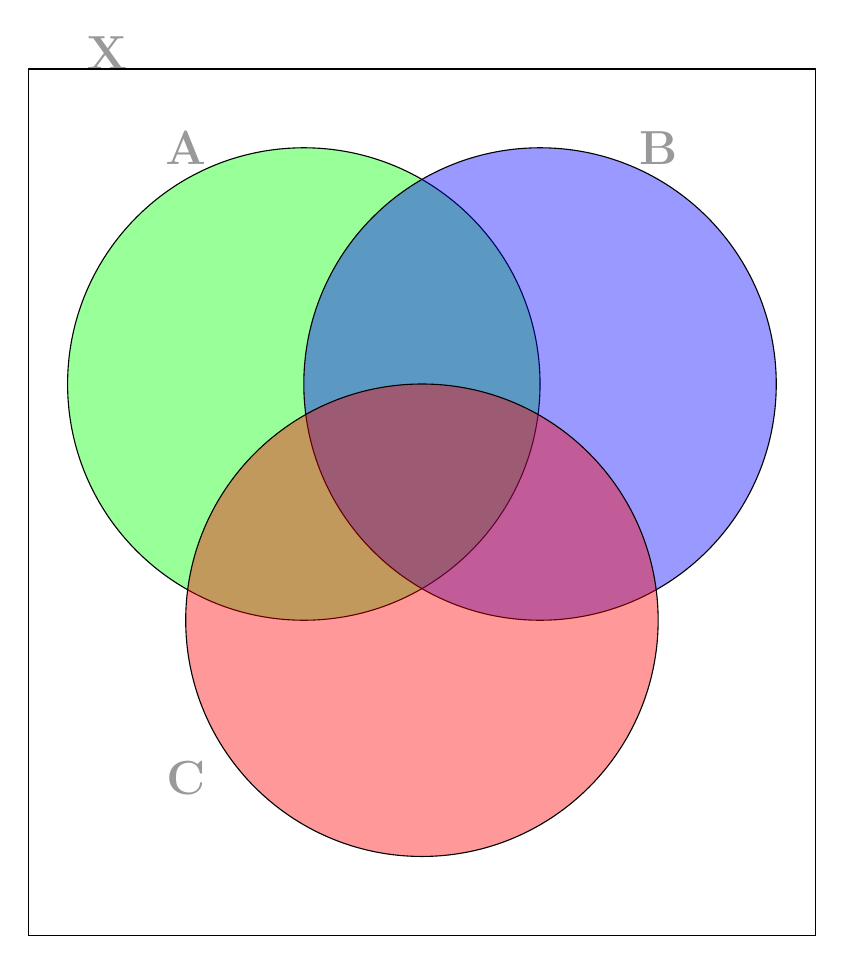
\begin{tikzpicture}
%% You can adjust the opacity here. For venn diagrams it is convenient to have a low opacity so that you can see intersections
	\begin{scope} [fill opacity = .4]
%% The draw command knows a lot of shapes. To make a rectangle you just need to specify two diagonal corners. Make sure you always have a semicolon at the end of your draw commands, otherwise latex flips out.
    \draw (-5,5) rectangle (5,-6);
%% Similarly, you can make a circle by specifying the center and then the radius. You can also add a fill color, but if you're printing in black and white you'll probably want to remove that line.
    \draw[fill=green, draw = black] (-1.5,1) circle (3);
    \draw[fill=blue, draw = black] (1.5,1) circle (3);
    \draw[fill=red, draw = black] (0,-2) circle (3);
%% We can use the node command to label points. If you put your cursor on "LARGE" or "textbf" a box will drop down with size and text style options.
    \node at (-4,5.2) {\LARGE\textbf{X}};
    \node at (-3,4) {\LARGE\textbf{A}};
    \node at (3,4) {\LARGE\textbf{B}};
    \node at (-3,-4) {\LARGE\textbf{C}};
    \end{scope}
%% And now you have a venn diagram. Yay!
%\draw[help lines](-5,5) grid (5,-6);    This line can draw the grid lines to help guide you. I use these when I'm writing the code and then delete this line when I publish the pdf.
\end{tikzpicture}


\end{document}
